\documentclass{article}
\usepackage{fullpage}
\usepackage{parskip}
\usepackage{hyperref}
\usepackage{listings}
\usepackage{graphicx}
\usepackage{amssymb}
\usepackage{mdwlist}
\usepackage{textcomp}
\usepackage[usenames,dvipsnames]{color}
\hypersetup{
    colorlinks,
    citecolor=Red,
    linkcolor=Red,
    urlcolor=Red}
\begin{document}

\title{Assignment 2: 3D Geometry, Lighting, and Shading}
\author{CS148 Fall 2015-2016}
\date{}
\maketitle

\section*{Introduction}

\begin{figure}[h!]
    \centering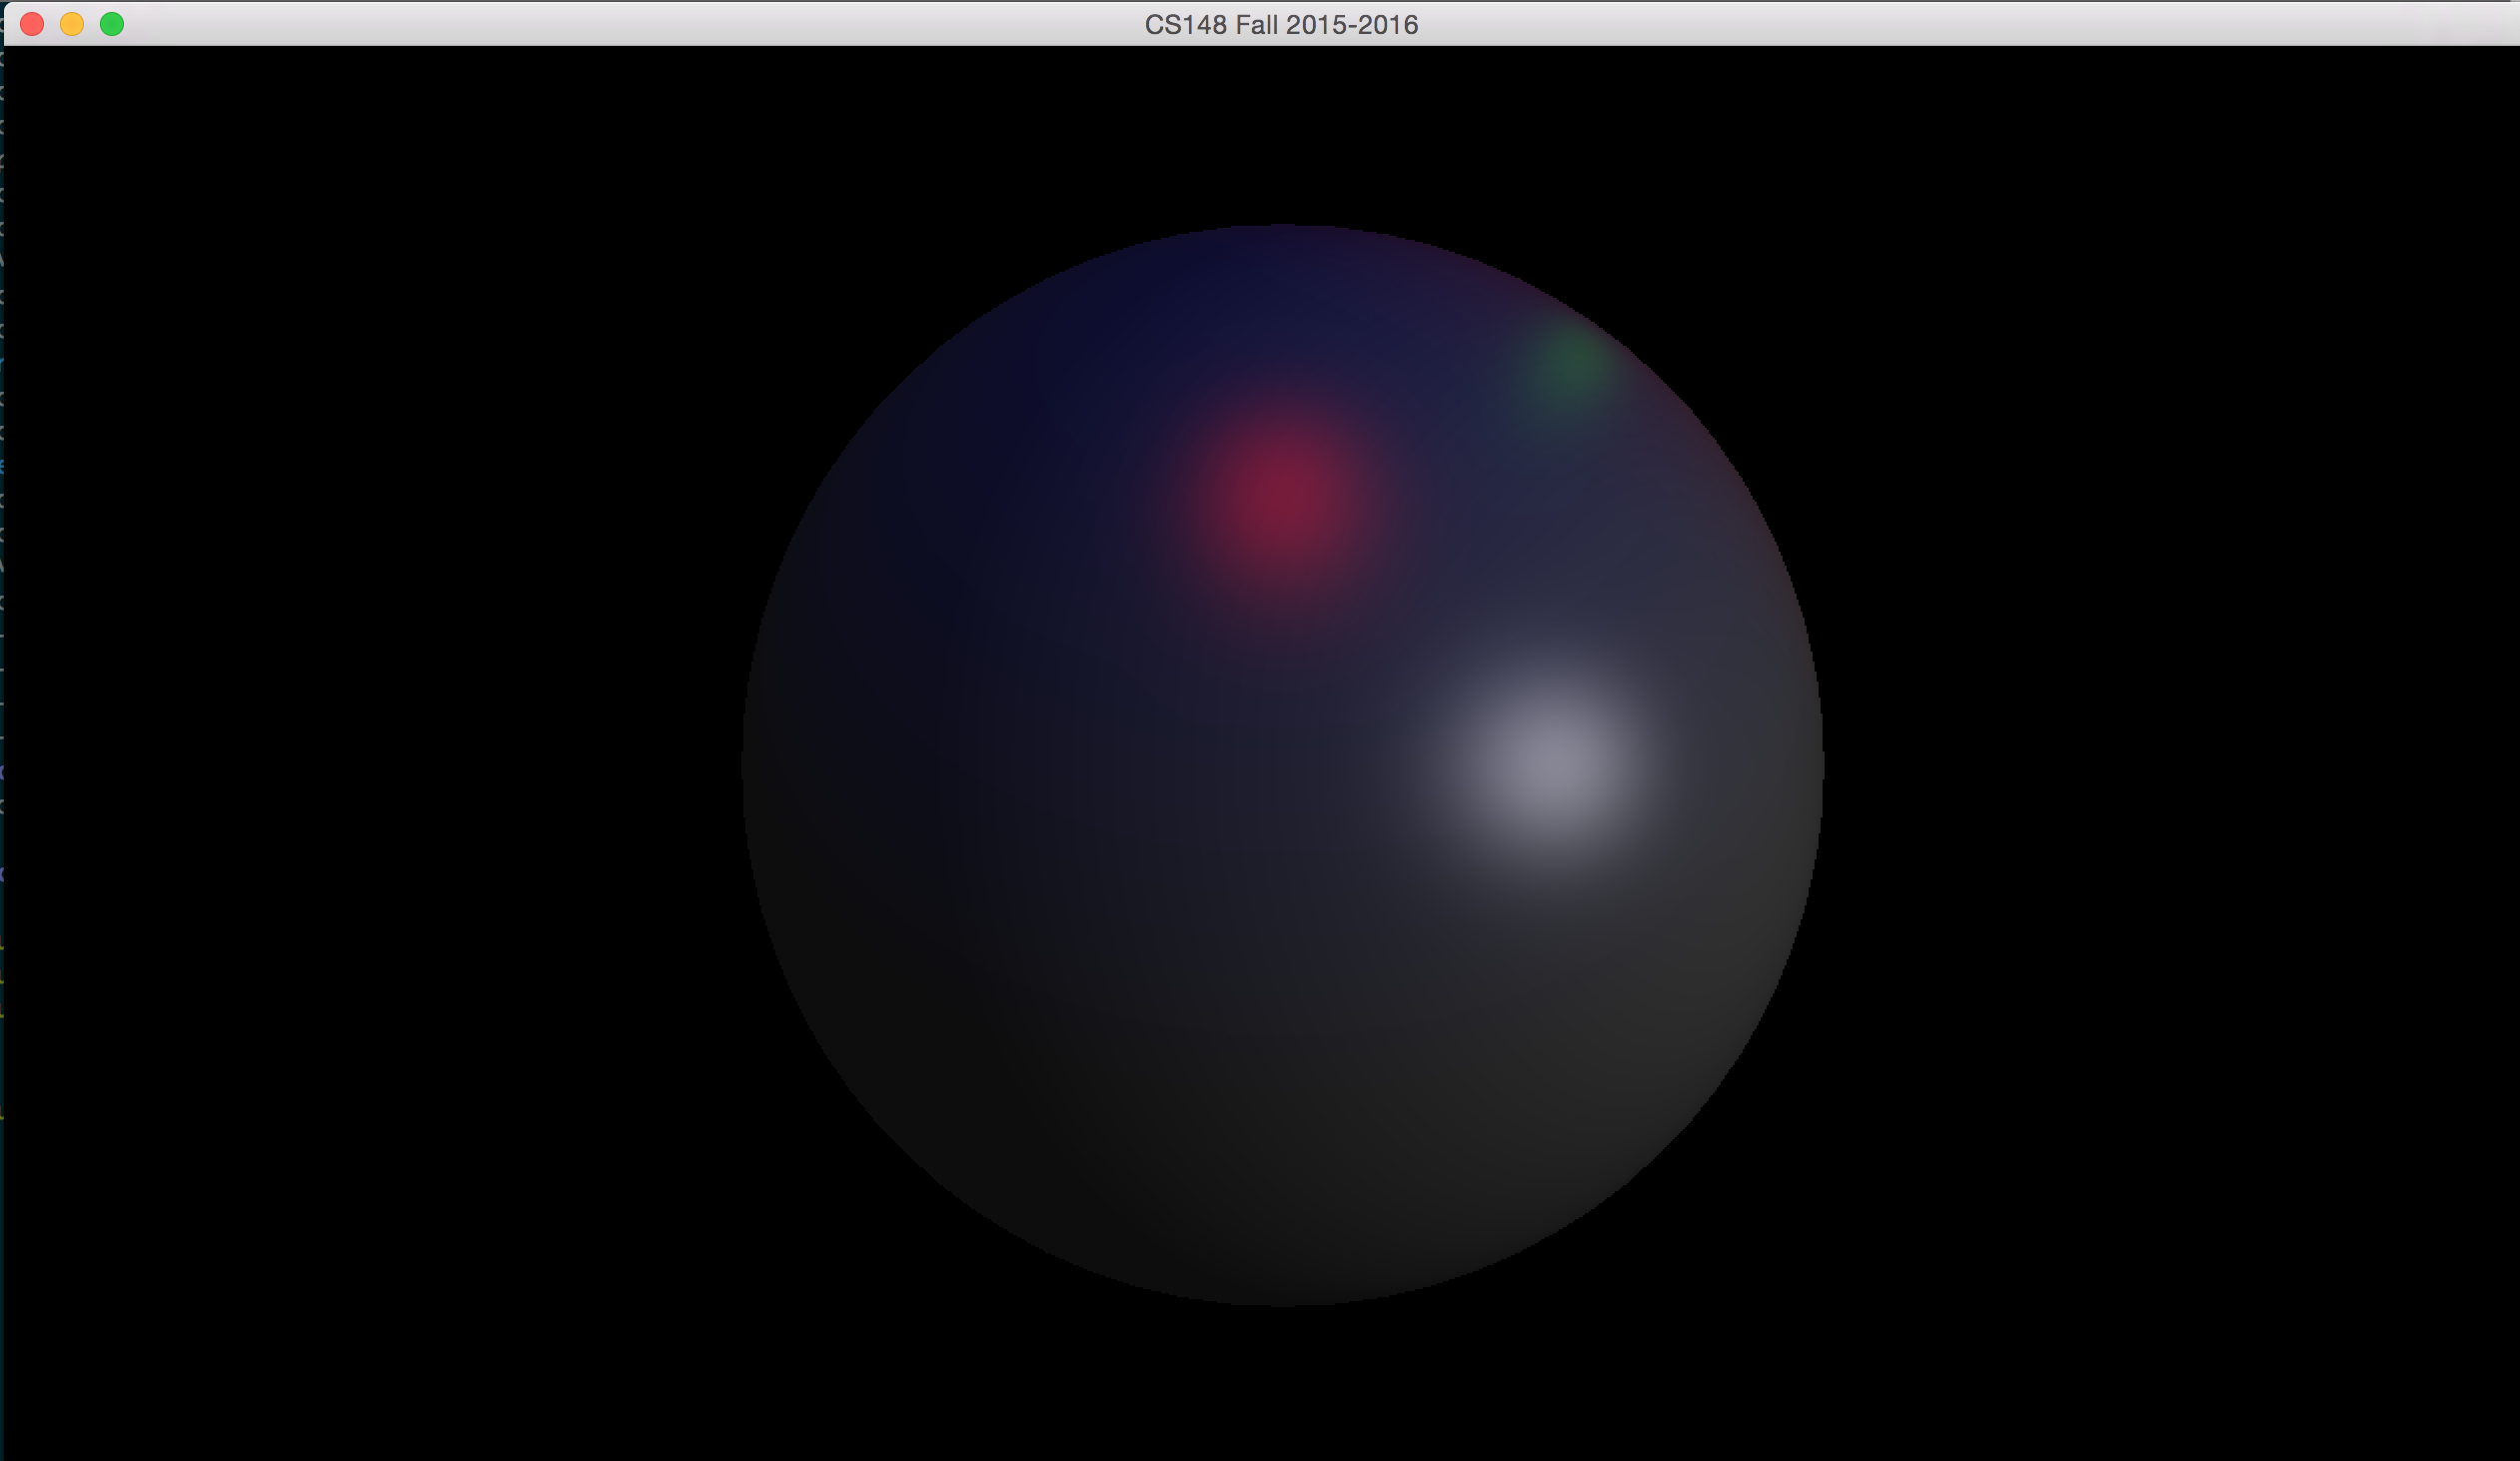
\includegraphics[width=0.7\linewidth]{assign2.png}
    \caption{A Sphere with Three Moving Lights using Blinn-Phong Shading}
\end{figure}

In this assignment we will explore the process of getting a 3D object onto the screen, lit, and shaded. You will also become more familiar with GLSL (the OpenGL shading language). Do note that there are many ways to light and shade a 3D scene! The method we chose in the assignment framework is just one way of doing so. Feel free to implement your own way of handling lights and creating your own shaders!

Finally, you will begin the process of creating your final image (for the OpenGL assignments)! You will need to find 3D geometry and place it in your scene, adjust the camera, and add and adjust lights to get a nice image! You may have to iterate this process many times until you get an image to your liking. Remembmer, start early and ask questions if you get stuck!

\subsection*{Useful Resources}

\begin{enumerate*}
    \item OpenGL Programming Guide Chapters 3-5, 7 (the book is not required, but recommended!)
    \item OpenGL 4 Documentation: \href{https://www.opengl.org/sdk/docs/man4/}{here}. Note that these pages are for OpenGL 4.5 but most should be equivalent (unless otherwise noted on the function's page).
    \item SDL 2 Documentation: \href{https://wiki.libsdl.org/CategoryAPI}{here}.
    \item GLSL Tutorial: \href{http://www.lighthouse3d.com/tutorials/glsl-tutorial/}{here}.
    \item GLM: \href{http://glm.g-truc.net/0.9.7/glm-0.9.7.pdf}{Manual} and \href{http://glm.g-truc.net/0.9.7/api/index.html}{Documentation}.
    \item C++ Reference: \href{http://en.cppreference.com/w/}{here}
    \item Open Asset Import Library Documentation: \href{http://assimp.sourceforge.net/lib_html/index.html}{here}
    \item Assignment Framework Documentation: This can be found in "source/doxygen"
\end{enumerate*}

\subsection*{Finding Meshes Online (For Free!)}
\begin{enumerate*}
    \item \href{http://www.turbosquid.com/}{TurboSquid}.
    \item \href{http://www.polycount.com/forum/}{PolyCount}. Note that it may be useful to Google "Polycount free models".
    \item \href{http://tf3dm.com/}{TF3DM}.
\end{enumerate*}

Note that it is hard to find high quality models and textures online. You may find it useful to look for people who have used "Zbrush" to create high-poly models and then trying to find a way to get an OBJ from that.

\subsection*{Creating your Own Meshes (For Free!)}
\begin{enumerate*}
    \item \href{http://www.autodesk.com/education/free-software/maya}{Autodesk Maya}
    \item \href{http://www.autodesk.com/education/free-software/3ds-max}{Autodesk 3ds Max}
    \item \href{https://www.blender.org/}{Blender}
\end{enumerate*}

I personally find Blender very hard and uninuitive to use (it has a pretty steep learning curve, in my opinion) compared to Maya and 3DS Max, but the choice is up to you! Additionally, you can generate your models procedurally in code.

\section*{Assignment}

In this assignment's code, you will see the use of "DISABLE\_OPENGL\_SUBROUTINES" which is only defined on Mac OS X. This is due to OpenGL subroutines being broken on Mac OS X (at least with a NVIDIA graphics card). This does not affect Windows and Linux users. As a result, I have two versions of the shaders used, one with subroutines and one without subroutines. If you are on Mac, make sure you look at/modify the shaders in the "noSubroutine" folders.

\subsection*{Assignment 2 Code Explanation}

Look in the Assignment2 class documentation in the assignment framework documentation found at "source/doxygen".

\subsection*{Asset Loading}

Assets (models, textures) are stored in the "assets" folder. When the program is configured and compiled, a C++ preprocessor definition is added to tell the program where to look for this folder. Much like the shaders, when you load an asset (whether it be a mesh or a texture), make sure the path is specified relative to the "assets" folder.

\subsection*{Pointers to Get You Started}
\begin{itemize*}
    \item The code to generate 'RenderingObject's from a file (OBJ, FBX, whatever) is found in "common/Utility/Mesh/Loading/MeshLoader.h/cpp". Note that we make use of the Open Asset Import Library which takes care of actually parsing the file; all we do is read in the data given to us by the library. Note that currently the LoadMesh function does not support reading in materials from the file so you will have to create the material parameters yourself!
    \item The shaders "shaders/brdf/blinnphong/vert" demonstrate Gouraud shading while the shaders in "source/shaders/brdf/blinnphong/frag" demonstrate Phong shading. Run the assignment to see the different between the two.
    \item The OpenGL shaders are tightly coupled to the corresponding shader class in the assignment framework. Look at the GLSL shaders found in "source/shaders/brdf/blinnphong/vert" (or frag) and look at "common/Rendering/Shaders/BlinnPhongShader.h/cpp" to see how certain variables correspond.
    \item We have provided an implementation of Blinn-Phong shading. You can read more about it \href{http://citeseerx.ist.psu.edu/viewdoc/download?doi=10.1.1.131.7741&rep=rep1&type=pdf}{here}. You may find the \href{https://en.wikipedia.org/wiki/Blinn%E2%80%93Phong_shading_model}{Wiki} to be more useful.
    \item The code has a distinction between a "Light" and its properties ("LightProperties"). "Light" will control physical properties such as its location, direction its facing, etc. "LightProperties" on the other hand will control the actual shading properties like its diffuse color, specular color, etc. As a result,  the type of "LightProperties" is dependent on which "ShaderProgram" subclass you use (i.e. BlinnPhongShader).
    \item As an addendum to the previous point, to add a new type of light (i.e. a directional light), you will want to have a subclass of "Light", add a new light type to "LightType" (in Light.h), and then make sure you handle the new type of light in BlinnPhongShader.cpp in the "SetupShaderLighting" function. In your new light class, make sure you call the Light constructor with the new enum type! Additionally, make sure you have everything setup in the GLSL shader to handle your changes. "SetShaderSubroutine" and "SetShaderUniform" will fail silently if they can't find something.
\end{itemize*}

\subsection*{Going Beyond the Assignment (Optional)}
\begin{itemize*}
    \item The type of rendering implemented currently is a multi-pass forward renderer. What this means is that for every object, we go through each light and run the vertex/fragment shader once. To compute the final image, we blend the colors together to get the final result! This technique does not scale, however. As the number of lights increases and as the complexity of the scene grows, your fragment shaders will be doing a lot of work (a lot of which is unnecessary). A solution to this is to use \href{https://en.wikipedia.org/wiki/Deferred_shading}{deferred shading}. 
    \item Try your hard at implementing even more advanced rendering techniques such as screen space ambient occlusion! \href{https://en.wikipedia.org/wiki/Screen_space_ambient_occlusion}{(Wiki Page)}.
    \item The Blinn-Phong reflection model isn't the only reflection model that exists! It is merely one example of a \href{https://en.wikipedia.org/wiki/Bidirectional_reflectance_distribution_function}{BRDF}. Check out Epic's shading presentation at SIGGRAPH 2013 to check out how they do shading in Unreal Engine 4 \href{http://blog.selfshadow.com/publications/s2013-shading-course/karis/s2013_pbs_epic_notes_v2.pdf}{here}. The Disney presentation they reference can be found \href{http://blog.selfshadow.com/publications/s2012-shading-course/burley/s2012_pbs_disney_brdf_notes_v3.pdf}{here}.
    \item Lighting does not look nice without shadows! Look into \href{https://en.wikipedia.org/wiki/Shadow_mapping}{shadow mapping}.
\end{itemize*}

\section*{Questions}
\begin{enumerate*}
    \item In the context of a vertex shader, what is the difference between a 'uniform' variable and a variable passed to the shader via the 'in' keyword.
    \item When would you expect diffuse lighting for a vertex to be strongest in Blinn-Phong shading (i.e. when X is pointing towards Y).
    \item What is the difference between a directional light and a point light?
\end{enumerate*}

\section*{Feedback (Optional)}
\begin{enumerate*}
    \item On a scale of 1-10 [10 being the most work]: How much work was this assignment?
    \item Do you wish the assignment framework abstracted less of the underlying OpenGL API? More? Just right?
\end{enumerate*}

\section*{Grading}
This assignment will be graded on the following requirements
\begin{itemize*}
    \item There are at least two different geometric models in your scene.
    \item There are at least two types of lights in the scene (i.e. a point light and a directional light).
    \item The student is able to adequetely answer questions asked by the CAs.
\end{itemize*}
according to the following rubric.
\begin{itemize*}
\item $+$ -- Exceeds the requirements via one or more artistic/technical contributions
\item $\checkmark$ -- Meets all of the requirements
\item $-$ -- Does not meet the requirements but still produces a drawing.
\item $0$ -- The submitted solution does not produce a drawing.
\end{itemize*}

\end{document}

